\documentclass{beamer}
\usepackage[utf8]{inputenc}
\usepackage{hyperref}
\usepackage{multicol}
\usepackage{hyperref}
\usepackage{graphicx}
\usepackage{booktabs}
\usepackage[font={small,it},labelfont=bf]{caption}

\DeclareMathAlphabet{\mathpzc}{OT1}{pzc}{m}{it}

\hypersetup{
    colorlinks=true,
    urlcolor={blue!40!black},
    linkcolor={red!50!black}
}

\inputencoding{utf8}

\mode<presentation> {
    \usetheme{Madrid}
}

\title{Logica de primer orden: Semantica}
\author{Prof. Ernesto Rodriguez}
\institute{
    Universidad del Itsmo \\
    \medskip \textit{erodriguez@unis.edu.gt}
}

\date[\today]{}

\begin{document}

\begin{frame}
\titlepage
\end{frame}

\begin{frame}
    \frametitle{El Triangulo de la Semantica}
    \begin{center}
    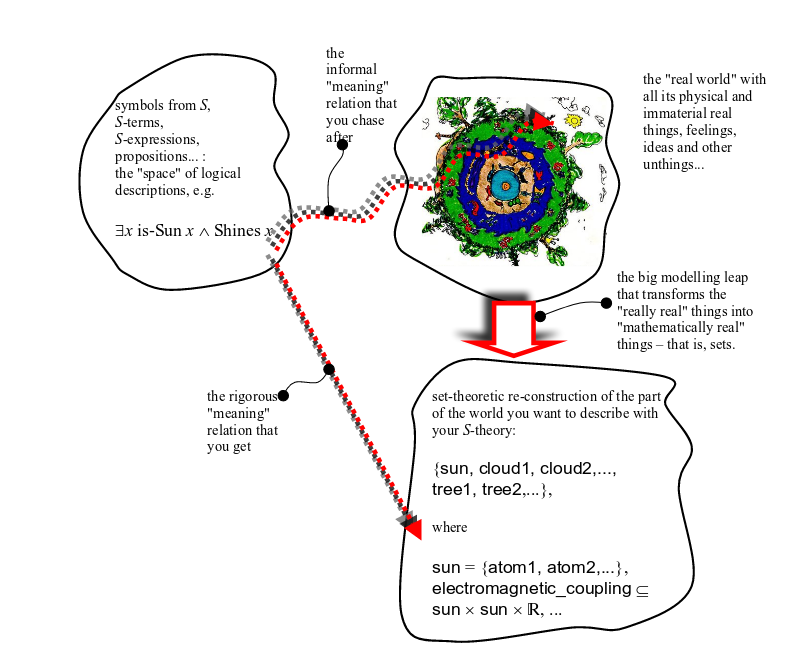
\includegraphics[width=8cm]{triangulo.png}
    \end{center}
    \tiny{Imagne obtenida de \cite{FLL}}
\end{frame}

\begin{frame}
    \frametitle{Semantica de la L\'ogica de Primer Orden}
    \begin{itemize}
        \item{El proposito de la l\'ogica es responder preguntas sobre alg\'un
            dominio}
        \item{Generalmente, ese dominio pertenece al mundo real, con todos sus
            objetos materiales, immateriales, sentimientos, ect.}
        \item{Sin embargo, la l\'ogica esta limitada a objetos que pueden existir
            en un pedazo de papel}
        \item{Por eso mismo, utiliza los conjuntos como sus objetos}
        \item{Debido a que el ``mundo real'' no esta hecho de conjuntos (abierto a discusi\'on filosofica),
            necesitamos modelar nuestro \emph{dominio de interes} mediante conjuntos}
        \item{A este \emph{dominio de interes} se le conoce como la \emph{Estructura-S}}
    \end{itemize}
\end{frame}

\begin{frame}
    \frametitle{La Estructura-S}
    {\bf Estructura-S:} Un conjunto que contiene todos los objetos con los que trabaja
    una l\'ogica de primer orden. Formalemente, para un conjunto $S$ de simbolos
    constantes, predicados y funciones, se define una \emph{Estructura-S} (denotada
    como $\mathpzc{A}$) es un conjunto $A$ (llamado el transportador de $\mathpzc{A}$)
    con las siguientes caracteristicas:
    \begin{itemize}
        \item{Por cada simbolo constante $c \in S$, existe un elemento en $c^\mathpzc{A}\in A$}
        \item{Por cada predicado unitario $\mathtt{P}\in S$, existe un conjunto $\mathtt{P}^\mathpzc{A}\subset A$}
        \item{Por cada predicado binario $\mathtt{R}\in S$, existe un conjunto $\mathtt{R}^\mathpzc{A}\in A\otimes A$}
        \item{Una funcion binaria $\mathit{f}\int S$ es una funcion cuyo dominio y rango pertenecen a $A$.
            Se puede definir como $\mathit{f}^\mathpzc{A}:=\{(x,y)|\mathit{f}(x)=y\}.$}
        \item{Los predicados y funciones de mayor aridad se definien de forma similar.}
    \end{itemize}
\end{frame}

\begin{frame}
    \frametitle{La Estructura-S}
    A menudo, los ingredientes de una \emph{Estructura-S} $\mathpzc{A}$ se colocan en
    una tupla. Por ejemplo:
    \begin{itemize}
        \item{Si nuestro conjunto $S$ de simbolos contiene $\{+,0,1\}$, podemos
            escribir $\mathpzc{A}:=(\mathbb{N}, +^{\mathbb{N}}, 0^{\mathbb{N}}, 1^{\mathbb{N}})$}
        \item{El el conjunto $S$ de numeros naturales ordenados $\{+,\mathtt{<},0,1\}$
            se escribe $\mathpzc{A}:=(\mathbb{N}, +^{\mathbb{N}}, \mathtt{<}^{\mathbb{N}}, 0^{\mathbb{N}}, 1^{\mathbb{N}})$}
    \end{itemize}
\end{frame}

\begin{frame}
    \frametitle{Observaciones}
    \begin{itemize}
        \item{La l\'ogica de primer orden (y las l\'ogica en general) obligan
            que uno describa su contenido antes de utilizarse.}
        \item{Si uno desea extender el dominio de una l\'ogica, uno debe definir
            nueva mente la \emph{Estructura-S}.}
        \item{En alg\'unos casos, se puede extneder el vocabulario definiendo nuevos
            simbolos mediante la l\'ogica misma. Por ejemplo: $\forall x\ 2=x\Leftrightarrow x=1+1$}
        \item{Puede succeder que la l\'ogica no sea una buena herramienta para describir
            procesos que ocurren a traves del tiempo. Por ejemplo, la evoluci\'on, donde
            nuevas especies aparecen y viejas especies de-aparecen.}
        \item{Existe la logica \emph{lineal-temporal} que permite describir procesos
            que ocurren a traves del tiempo.}
    \end{itemize}
\end{frame}

\begin{frame}
    \frametitle{Interpretaciones}
    \begin{itemize}
        \item{ Una interpretaci\'on $\mathcal{I}$ es una pareja $(\mathpzc{A}, \beta)$ donde
            $\mathpzc{A}$ es una \emph{Estructura-S} y $\beta$ es una asignaci\'on de variables.}
        \item{Una asignaci\'on de variables es un diccionario que para toda variable $x$,$y$,$z$, etc.
            define un objeto $c\in A$ al cual apunta la variable.}
    \end{itemize}
\end{frame}

\begin{frame}
    \frametitle{Re-asignaci\'on de Variables}
    Dada una asignaci\'on de variables $\beta$ se define la re-asignaci\'on
    de variables $\beta \frac{a}{x}$ como una asignaci\'on que actua igual a
    $\beta$ excepto en el caso de $x$, a la cual se le asigna el valor $a$:
    \[
        \beta \frac{a}{x}(y)=
        \left\{
            \begin{array}{ll}
                a  & \mbox{if } y = x \\
                \beta(y) & \mathtt{otherwise}
            \end{array}
        \right.
    \]
    Dado $\mathcal{I}:=(\mathpzc{A},\beta)$, tambi\'en se define $\mathcal{I}\frac{a}{x}$
    como $(\mathpzc{A}, \beta\frac{a}{x})$
\end{frame}

s\begin{frame}
    \frametitle{Interpretaci\'on de Expressiones}
    Ahora, dada una expression y una interpretaci\'on $\mathcal{I}:=(\mathpzc{A},\beta)$,
    podemos interpretarla de la siguiente manera:
    \begin{itemize}
        \item{Para toda variable $x$, $\mathcal{I}(x)=\beta(x)$}
        \item{Dada una constante $\mathtt{c}\in S$, $\mathcal{I}(\mathtt{c})=\mathtt{c}^{\mathpzc{A}}$}
        \item{Dado $\mathit{f}$ y las expressiones $x_1,\ldots,x_n$:
            $\mathcal{I} (\mathit{f} x_1,\ldots ,x_n) = \mathit{f}^{\mathpzc{A}}(\mathcal{I}(x_1),\ldots\mathcal{I}(x_n))$}
    \end{itemize}
\end{frame}

\begin{frame}
    \frametitle{Relaci\'on de Modelado}
    Dada una interpretaci\'on $\mathcal{I}=(\mathpzc{A},\beta)$ y una
    expression $\varphi$, podemos definir la \emph{relacion de modelado} $\mathcal{I}\models\varphi$
    (dicho $\mathcal{I}$ es un modelo de $\varphi$) como:
    \\\vspace{0.5cm}
    \begin{tabular}{l l l}
        $\mathcal{I} \models t_0=t_1$ & si & $\mathcal{I}(t_1)=\mathcal{I}(t_2)$ \\
        $\mathcal{I} \models \mathtt{R}\ t_1,\ldots,t_n$ & si & $\mathcal{I}(t_1)\otimes,\ldots,\otimes\mathcal{I}(t_n) \in \mathtt{R}^\mathpzc{A}$\\
        $\mathcal{I} \models \neg \varphi$ & si no & $\mathcal{I} \models \varphi$\\
        $\mathcal{I} \models \varphi\wedge\psi$ & si & $\mathcal{I}\models\varphi$ and $\mathcal{I}\models\psi$\\
        $\mathcal{I} \models \varphi\vee\psi$ & si & $\mathcal{I}\models\varphi$ or $\mathcal{I}\models\psi$ \\
        $\mathcal{I} \models \forall x \varphi$ & si & para todo $a \in A$, $\mathcal{I}\frac{a}{x}\models\varphi$ \\
        $\mathcal{I} \models \exists x \varphi$ & si & existe alg\'un $a \in A$, $\mathcal{I}\frac{a}{x}\models\varphi$
    \end{tabular}

    \vspace{0.5cm}
    Las reglas para ($\Leftarrow$) y ($\Leftrightarrow$) se pueden definir de la misma forma.
\end{frame}

\begin{frame}
    \frametitle{Relaci\'on de Modelado}
    \begin{itemize}
        \item{Una expresi\'on $\varphi$ solo puede ser cierta o mentira
            respecto a alguna interpretaci\'on $\mathcal{I}$}
        \item{Las interpretaci\'ones $\mathcal{I}$ nos permiten colocar
            objetos matematicos dentro de formulas logicas.}
        \item{La importancia de esta relaci\'on entre formulas y objetos
            sera m\'as clara cuando estudiemos un calculo que nos permite
            trabajar on dichas formulas.}
    \end{itemize}
\end{frame}

\begin{frame}
    \frametitle{Vinculaci\'on}
    {\bf Relaci\'on de Vinculaci\'on}: Dada una expresi\'on $\varphi$ y
    un conjunto $\phi$, escribimos $\phi\models\varphi$ (dicho $\phi$
    vincula a $\varphi$) si toda interpretaci\'on que es un modelo
    de $\phi$ (es decir que es un modelo para todo $\psi\in\phi$)
    tambien es un modelo de $\varphi$.
    \\\vspace{1cm}
    \begin{itemize}
        \item{La \emph{Relacion de Vinculaci\'on} es en essencia una ``verdad matematica''
            ya que dice que dada una serie de suposiciones ($\phi$) poemos ver que
            $\varphi$ es cierto.}
        \item{Una \emph{Relacion de vinculaci\'on} simpre existe o no, sin importar
            si alguien ya lo demostro o no.}
    \end{itemize}
\end{frame}

\begin{frame}
    \frametitle{Formalidades}
    \begin{itemize}
        \item{Una expresi\'on $\varphi$ es una tautologia, si la
        vincula el conjunto vacio ($\emptyset\models\phi$). Ej.
        $\forall x\ \neg\neg x \Leftrightarrow x$}
        \item{Una expresi\'on $\varphi$ es \emph{invalida} o una \emph{contradicci\'on}
            si no existe un conjunto $\phi$ tal que $\phi\models\varphi$}
        \item{Una expresi\'on $\varphi$ es satisfacible si existe al\'un $\phi$
            tal que $\phi\models\varphi$}
        \item{Dos expresiones $\varphi$ y $\psi$ son equivalentes si $\varphi\models\psi$
            y $\psi\models\varphi$, tambien escrito como $\varphi\Leftrightarrow\psi$}
    \end{itemize}
\end{frame}

\begin{frame}
    \frametitle{Referencias}
    \bibliography{../Referencias/referencias}
    \bibliographystyle{plain}
\end{frame}

\end{document}